\documentclass[12pt,a4paper,ngerman]{report}
\usepackage{babel}
%\usepackage{natbib}
\usepackage{url}
%\usepackage[left=2cm, right=1.5cm, top=2cm, bottom=2cm]{geometry}
%\usepackage[ansinew]{inputenc}
\usepackage{amsmath}
\usepackage{nicefrac} % macht schöne Brüche mit querstrich mit \nicefrac{1}{2}
\usepackage{graphicx}
%\graphicspath{}
\usepackage{titlesec}% um chapterüberschriften anzupassen.
\titleformat{\chapter}{\normalfont\huge\bf}{\thechapter.}{20pt}{\huge\bf}
\usepackage{parskip}
\usepackage{fancyhdr}
\usepackage{amsfonts}
\usepackage{float}
\usepackage{caption}
\usepackage{subcaption} % for \begin{subfigure}
	
\usepackage{csquotes} % mit \enquote{blabla} tolle anfürungsstriche erstellen
%\usepackage{physics} %lässt mich \bra und \ket benuzen %im konflict mit siunitx

\usepackage{pgfplots} %für plots
\pgfplotsset{compat=newest}

\usepackage{varioref} % macht mit \vref{} viel bessere referenzen
\usepackage{hyperref} % macht klickbare referenzen

\usepackage{xcolor, soul} %mit \hl{} kann man toll Sachen hervorheben.
\newcommand{\highlight}[1]{%
	\colorbox{yellow!50}{$\displaystyle#1$}} % mit \highlight{} kann man sogar in Gleichungen hervorheben

\usepackage{vmargin}
\usepackage[section]{placeins}
\usepackage{capt-of}
\usepackage{enumitem}
\usepackage{multirow}
\usepackage{blindtext}
\usepackage[version=4]{mhchem} % um Chemische Elementsymbole zu benutzen: \ce{H20}

\usepackage{pdfpages} % um PDFs einzufügen

%spread to latex:
\usepackage{booktabs, multirow} % for borders and merged ranges
\usepackage{changepage,threeparttable} % for wide tables

\providecommand{\e}[1]{\ensuremath{\cdot 10^{#1}}}
\providecommand{\fehlt}{\textcolor{red}{{ ¡Fehlt! }}}

\providecommand{\versuchstitel}{Perowskitsolarzellen} % Hier den Versuchstitel eintragen!

\usepackage{siunitx}
\sisetup{
	separate-uncertainty = true,
	%per-mode = fraction,
	%per-mode = symbol
}
\DeclareSIUnit\bar{bar}
\DeclareSIUnit\atomicmassunit{u}
\usepackage{isotope}


\setmarginsrb{3 cm}{2.5 cm}{3 cm}{2.5 cm}{1 cm}{1.5 cm}{1 cm}{1.5 cm}
\title{\versuchstitel}


\author{Frederik Uhlemann, Florian Adamczyk}
% Author
\date{\today}
% Date

\makeatletter
\let\thetitle\@title
\let\theauthor\@author
\let\thedate\@date
\makeatother

\pagestyle{fancy}
\fancyhf{}
\rhead{\theauthor}
\lhead{\versuchstitel}
\cfoot{\thepage}
%%%%%%%%%%%%%%%%%%%%%%%%%%%%%%%%%%%%%%%%%%%%
\begin{document}
		
	%%%%%%%%%%%%%%%%%%%%%%%%%%%%%%%%%%%%%%%%%%%%%%%%%%%%%%%%%%%%%%%%%%%%%%%%%%%%%%%%%%%%%%%%%
	
	\begin{titlepage}
		\centering
		\vspace*{0.5 cm}
		% \begin{large} Justus-Liebig-Universität\\ Gießen \end{large}
		
\includegraphics[width = 0.6 \textwidth]{JLU_Giessen-Logo}	%University Logo
		\\[2.0 cm]
		% \begin{center}    \textsc{\Large Justus - Liebig - Universität}\\{Giessen}\\[0.8cm]	\end{center}% University Name
		Versuch 6 des\\
		\textsc{\Large Fortgeschrittenen-Praktikums}\\ [0.3 cm]				% Course Code
		\rule{\linewidth}{0.2 mm} \\[0.4 cm]
		{ \huge \bfseries \thetitle}\\%%% TITEL HERE
		\rule{\linewidth}{0.2 mm}\\
		Versuchstermin 21.6.2024 \\
		~ \\
		[2.0 cm]
		
		
		\begin{minipage}{0.49\textwidth}
			\begin{flushleft}
				 \emph{Praktikumsbetreuer:}\\
				 M.Sc. Tim P. Schneider\\
				 %  Affiliation\\
				 \small{\href{mailto:tim.schneider@ap.physik.uni-giessen.de}{tim.schneider@ap.physik.uni-giessen.de}}
			\end{flushleft}
		\end{minipage}~
		\begin{minipage}{0.49\textwidth}
			\begin{flushright}
				\emph{Protokoll von:} \\
				
				\large{Frederik Uhlemann}\\
				\small{\href{mailto:frederik-vincent.uhlemann@physik.uni-giessen.de}{frederik-vincent.uhlemann@physik.uni-giessen.de}\\~\\
					%Matrikel Nr.: \:  \\[0.5cm]
					%\href{mailto:}{}
				}
				\large{Florian Adamczyk} \\
				\small{\href{mailto:florian.marius.adamczyk@physik.uni-giessen.de}{florian.marius.adamczyk@physik.uni-giessen.de}\\
					%Matrikel Nr.: \: 8105234}
			}
		\end{flushright}
	\end{minipage}
	
	\end{titlepage}
	
%%%%%%%%%%%%%%%%%%%%%%%%%%%%%%%%%%%%%%%%%%%%%%%%%%%%%%%%%%%%%%%%%%%%%%%%%%%%%%%%%%%%%%%%%
\setcounter{secnumdepth}{2}
\setcounter{tocdepth}{3}
\tableofcontents
%\newpage

%%%%%%%%%%%%%%%%%%%%%%%%%%%%%%%%%%%%%%%%%%%%%%%%%%%%%%%%%%%%%%%%%%%%%%%%%%%%%%%%%%%%%%%%%
%\renewcommand{\thesection}{\arabic{section}} %lässt in den subsections die erste zahl von darüberliegenden chapter weg.

%\pagebreak
	
%\setcounter{chapter}{-1}
\chapter*{Einleitung}\addcontentsline{toc}{chapter}{Einleitung}
Im Rahmen dieses Versuchs steht die Herstellung und Untersuchung von Perowskitsolarzellen im Mittelpunkt, einem vielversprechenden und aktuellen Thema in der Photovoltaikforschung. Der Versuch bietet eine spannende Gelegenheit, tief in die Welt der modernen Solarzellen einzutauchen und ein besseres Verständnis für die Technologien zu gewinnen, die unseren Alltag nachhaltig beeinflussen.

Es geht darum, eine Perowskitsolarzelle herzustellen und deren Eigenschaften zu analysieren. Zunächst wird auf einem transparenten leitfähigen Oxid (TCO) eine Titandioxidschicht präpariert. Diese Schicht dient als Grundlage für die lichtabsorbierende Methylammoniumbleiiodid-Schicht, die wiederum von einem Lochtransportmaterial überdeckt wird. Dieser mehrschichtige Aufbau ist entscheidend für die Effizienz der Solarzelle und ihre Fähigkeit, Sonnenlicht in elektrische Energie umzuwandeln.

Die optischen Eigenschaften der Perowskitschicht werden anschließend im UV-Vis-Spektrometer untersucht. Diese Analyse ermöglicht es, das Absorptionsverhalten und die Lichtdurchlässigkeit der Schicht zu verstehen, was für die Optimierung der Solarzelle von großer Bedeutung ist. Ein weiterer wichtiger Aspekt des Versuchs ist die Messung des Verhaltens von Strom und Spannung der gesamten Solarzelle unter Bestrahlung mit Weißlicht unterschiedlicher Intensitäten. Diese Messungen sind entscheidend, um die Leistungsfähigkeit der Solarzelle zu bewerten und ihre Effizienz zu bestimmen.

Perowskitsolarzellen sind aufgrund ihrer hohen Effizienz und vergleichsweise geringen Herstellungskosten von großem Interesse für die Forschung und Industrie. Ihre Entwicklung könnte einen bedeutenden Beitrag zur Energiewende und zur Reduktion der \ce{CO2}-Emissionen leisten, indem sie eine kostengünstige und effiziente Alternative zu herkömmlichen Silizium-Solarzellen bieten. Damit bietet dieser Versuch nicht nur einen tiefen Einblick in die Funktionsweise und Herstellung von Perowskitsolarzellen, sondern zeigt auch deren enormes Potenzial für eine nachhaltige Energiezukunft auf. Dies macht den Versuch nicht nur wissenschaftlich relevant, sondern auch äußerst bedeutsam für den Alltag und die zukünftige Energieversorgung.

	% notiz an mich: mit "~ bewirke ich einen geschützten bindestrich an dem nicht getrennt werden darf.
	% nur eine ~ macht ein geschütztes (normales) Leerzeichen. \, macht ein halbes geschütztes Leerzeichen.

\chapter{Theorie}
	\section{Kenngrößen von Solarzellen}\label{ch:Kenngrößen}
	Als wird folgend auf die Grundsätzlichen Eigenschaften von Solarzellen eingegangen, damit die Eigenschaften der hergestellten Perowskitsolarzelle eingeordnet werden können.\\
	\begin{figure}[ht]
		\centering
		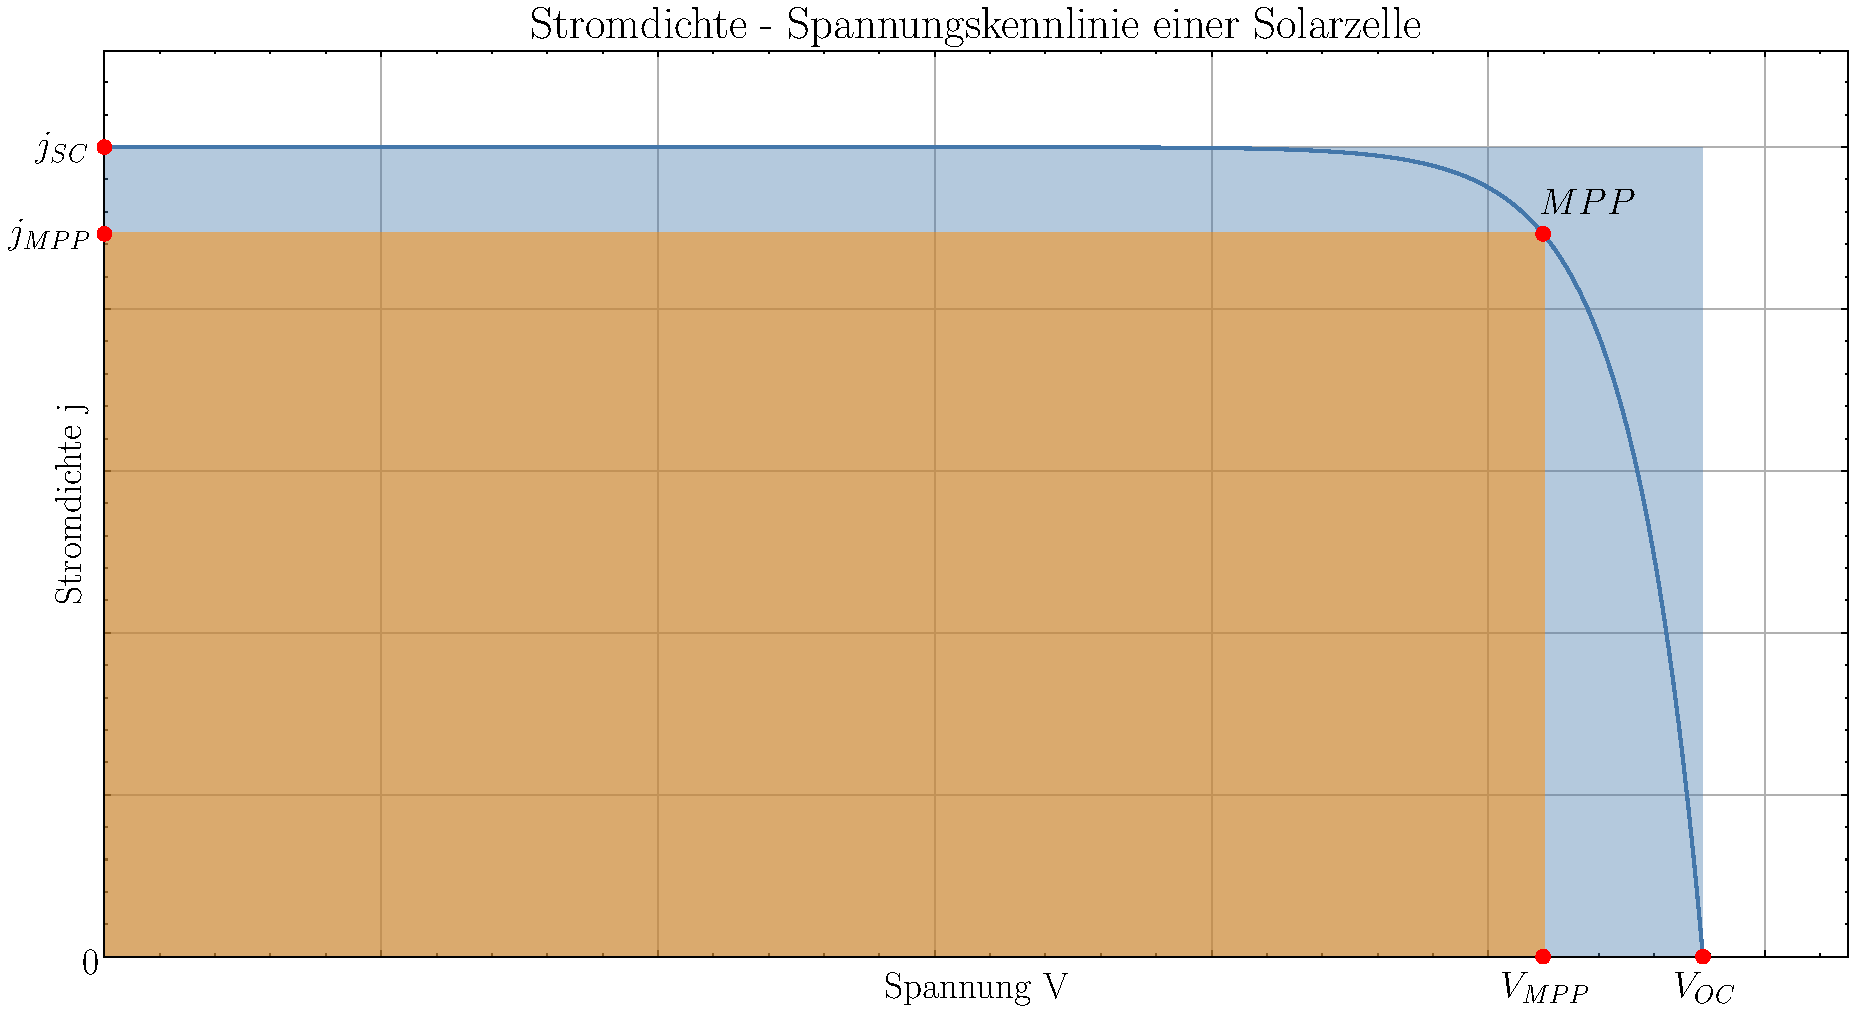
\includegraphics[width=\textwidth]{Bilder/SolarzelleIdeal.pdf}		
		\caption[Kennlinie ideale Solarzelle]{Stromdichte - Spannungskennlinie einer idealen Solarzelle, eingetragen sind zusätzlich wichtige Kenngrößen}
		\label{img:SolarzelleIdeal}
	\end{figure}
	Eine allgemeine Solarzelle verhält sich elektronisch ähnlich, wie eine Halbleiterdiode. In Abbildung \ref{img:SolarzelleIdeal} ist eine Solarzellenkennlinie abgebildet, der Unterschied zur Diodenkennlinie liegt allein in der Verschiebung in y-Richtung durch den Wert des Photostroms $j_{ph}$. Aus diesem Grund ist auch die Formel für die Stromcharakteristik bis auf diesen Wert identisch:
	\begin{equation}\label{eq:kennlinie}
		j(V) =  j_S \left(\text{exp}\left(\frac{e V}{m k_B T}\right) - 1\right) - j_{ph}
	\end{equation} 
	Der Photostrom kann für Perowskitsolarzellen folgendermaßen ausformuliert werden:
	\begin{equation}
		j_{ph} = e I_0 \eta_{CC} \eta_{inj} (1-\text{exp}(-\alpha d))
	\end{equation}
	Die dabei bisher aufgetretenen Variablen sind:
	\begin{itemize}
		\item Spannung $V$
		\item Sättigungsstromdichte $j_S$
		\item Elementarladung $e$ und Boltzmannkonstante $k_B$
		\item Idealitätsfaktor $m$
		\item Temperatur $T$
		\item Intensität des einfallenden Lichts $I_0$
		\item Effizienz für erzeugte Löcher/Elektronen transportierende Schichten zu erreichen $\eta_{CC}$
		\item Effizienz für Löcher/Elektronen in die Schichten einzutreten $\eta_{inj}$
		\item Absorptionskoeffizient $\alpha$
		\item Dicke der absorbierenden Schicht $d$
	\end{itemize}
	Nach dieser kurzen Einführung können die typischen Kenngrößen von Solarzellen erläutert werden.

	\paragraph{Kurzschlussstromdichte $j_{SC}$}
	Die Kurzschlussstromdichte ist gerade die Stromdichte bei einer Spannung von \SI{0}{\volt}, bei Belichtung einer Solarzelle. Sie ist in Abbildung \ref{img:SolarzelleIdeal} eingetragen, und entspricht dem Schnittpunkt mit der y-Achse der Kennlinie. Deshalb lässt sie sich folgend berechnen:
	\begin{equation}
		j_{SC} = j(V = 0) = e I_0 \eta_{CC} \eta_{inj} (1-\text{exp}(-\alpha d)) = j_{ph}
	\end{equation}
	\paragraph{Leerlaufspannung $V_{OC}$}
	Die Leerlaufspannung ist die Spannung bei einem Strom von \SI{0}{\ampere}, sie ist daher im Kennlinienfeld \ref{img:SolarzelleIdeal} als Nullstelle zu finden. Sie kann erneut aus der Gleichung \ref{eq:kennlinie} bestimmt werden:
	\begin{equation}
		\begin{split}
			 0 \overset{!}{=}  j_S \left(\text{exp}\left(\frac{e V_{OC}}{m k_B T}\right) - 1\right) - j_{ph}  \\
			 j_{ph} = j_S \, \text{exp}\left(\frac{e V_{OC}}{m k_B T}\right) \\
			 \Rightarrow V_{OC} = \text{ln} \left( \frac{j_{ph}}{j_S}\right) \frac{m k_B T}{e}
		\end{split}
	\end{equation} 
	Dabei wurde angenommen, dass $\text{exp}\left(\frac{e V_{OC}}{m k_B T}\right) \gg 1 $ und die Sättigungsstromdichte $j_{SC}$ entspricht gerade der Kurzschlussstromdichte $j_{SC}$, wie im Abschnitt davor gezeigt.
	\paragraph{Wirkungsgrad $\eta$}
	In der Abbildung \ref{img:SolarzelleIdeal} ist der sogenannte Maximum Power Point (MPP) eingetragen, er ist dort definiert, wo das Produkt aus der Stromdichte $j$ und der Spannung $V$ maximal ist. Die orangefarbene Fläche mit diesem Punkte, ist die maximale Leistungsdichte. Der Wirkungsgrad ist daher, dass Verhältnis aus dieser maximalen Leistungsdichte zur Leistungsdichte des eingestrahlten Lichts:
	\begin{equation}
		\eta = \frac{p_{max}}{p_0} = \frac{V_{MPP} \cdot j_{MPP}}{p_0}
	\end{equation}
	\paragraph{Füllfaktor FF}
	Aus den bisher beschriebenen Kenngrößen, kann der Füllfaktor angegeben werden, in der Abbildung .\ref{img:SolarzelleIdeal} ist eher das Verhältnis des orangen Rechtecks zum blauen Rechteck. Dieser Faktor gibt demnach das Verhältnis der Maximalleistung zur Leerlaufleistung an:
	\begin{equation}
		FF = \frac{V_{MPP} \cdot j_{MPP}}{V_{OC} \cdot j_{SC}}
	\end{equation}  

	\section{Aufbau einer Perowskitsolarzelle}
		\begin{figure}[ht]
		\centering
		\includegraphics[width=\textwidth]{Bilder/AufbauZelle.pdf}		
		\caption[Aufbau der Perowskit-Solarzelle]{Schematischer Aufbau der Perowskit-Solarzelle}
		\label{img:AufbauZelle}
	\end{figure}
	In Abbildung \ref{img:AufbauZelle} ist schematisch der schichtweise Aufbau einer Perowskit-Solarzelle abgebildet. Die einzelnen Schichten werden folgend von unten nach oben erläutert:
	\paragraph{Substrat}
	Die Solarzelle wird nach der Abbildung von der Unterseite beleuchtet, deshalb müssen die ersten Schichten transparent sein. Die erste Glas Schicht bildet eine stabile Unteralge für den Aufbau, dabei ist das Glas mit einem transparenten und leitfähigem Oxid beschichtet. zum Beispiel wird Fluordotiertes Zinnoxid (FTO) verwendet, dieses transportiert die entstehende Ladung zu einer Elektrode.
	\paragraph{n-leitende Schicht}
	Es folgt eine n-leitende Schicht, sie muss ebenfalls transparent sein und transportiert die in der Perowskitschicht entstehenden Elektronen ab. Häufige Verwendung findet hier Titanoxid \ce{TiO_{2}}.
	\paragraph{Perowskitschicht}
	In der Perowskitschicht werden Elektronen durch einstrahlende Photonen in das Valenzband gehoben, deshalb ist wichtig, dass diese Schicht einen hohen Absorptionskoeffizienten besitzt. In diesem Versuch wird Methylammoniumbleiiodid \ce{CH_3NH_3PbI_3} verwendet, es kristallisiert bei über \SI{60}{\celsius}, die dabei entstehende Kristallstruktur ist in Abbildung \ref{img:PerwoskitZelle} dargestellt. Zudem besitzt dieses Perowskit halbleitende Eigenschaften, da es eine direkte Bandlücke mit \SI{1.55}{\eV} aufweist.
	\begin{figure}[ht]
		\centering
		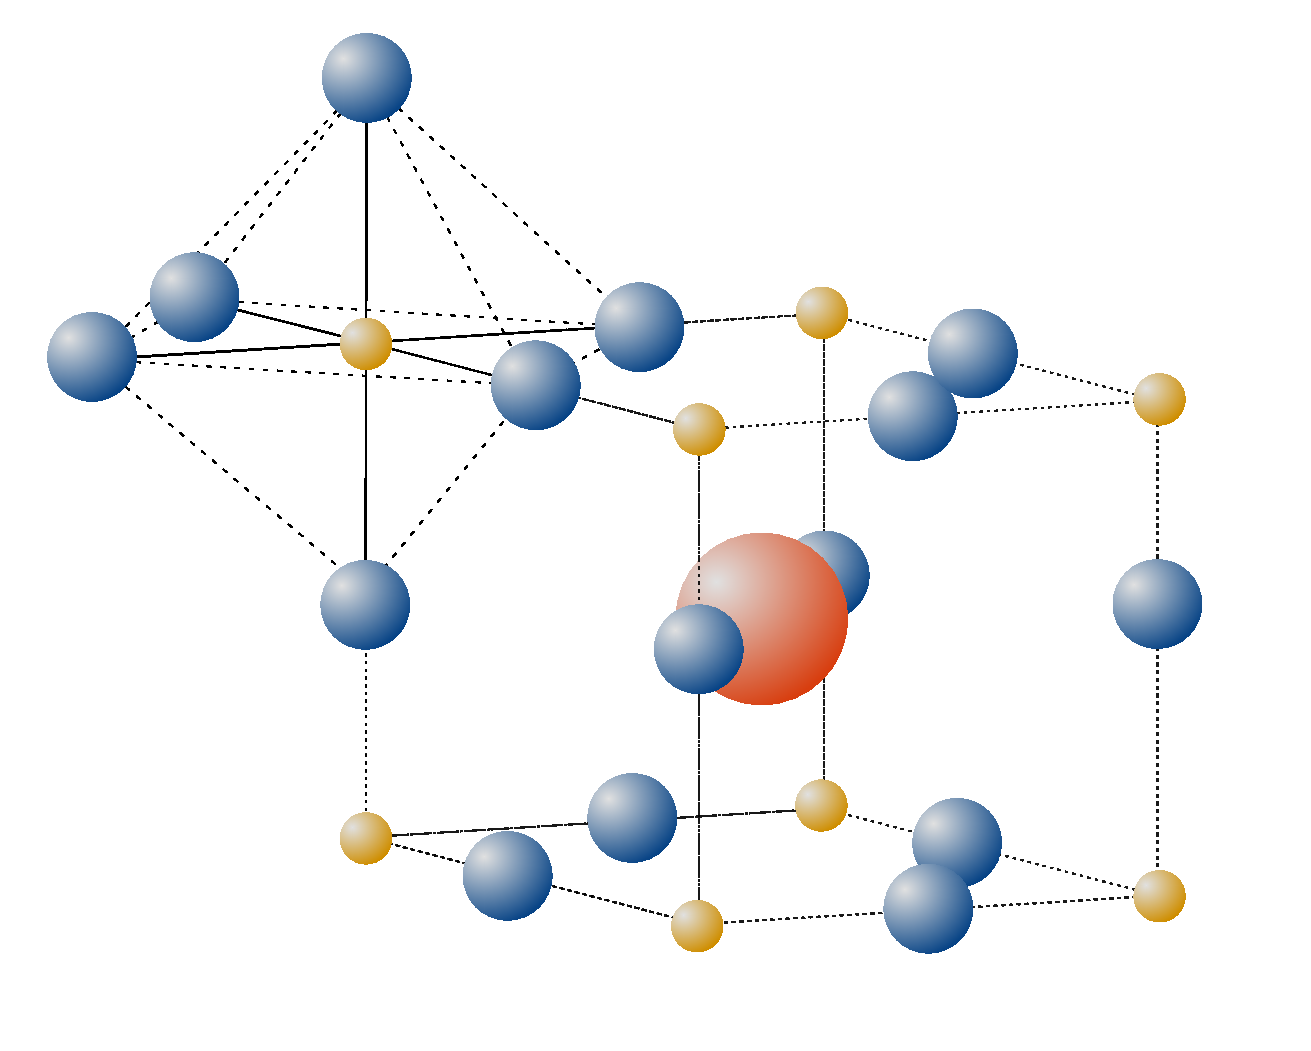
\includegraphics[width=\textwidth]{Bilder/PerwoskitZelle.pdf}		
		\caption[Einheitszelle von \ce{CH_3NH_3PbI_3}]{Einheitszelle des Methylammoniumbleiiodid, in Rot das organische Kation, Blau das Blei-Anion und gelb das Halogen-Ion}
		\label{img:PerwoskitZelle}
	\end{figure}
	\paragraph{p-leitende Schicht}
	Diese Schicht transportiert die entstehenden Löcher ab, dafür wird Kupferthiocyanat \ce{CuSCN} verwendet
	\paragraph{Gegenelektrode}
	Damit eine elektrischer Stromkreis geschlossen werden kann,folgt nun eine Schicht, welche die Löcher zur Gegenelektrode transportiert. Hier sind verschiedenste leitende Materialien verwendbar, im Versuch wird eine Kohlenstoffschicht verwendet.
	\paragraph{Substrat}
	Zuletzt folgt erneut das Substrat vom Anfang aus Glas und FTO, um die Solarzelle zu stabilisieren und einen äußeren Gegenelektrodenktontakt herzustellen.
	
		



	

\chapter{Versuchsdurchführung}
	\paragraph*{Sicherheitsmaßnahmen}
	Bevor mit dem Versuch begonnen wird, ist es notwendig, sich mit den Sicherheitsdatenblättern der verwendeten Chemikalien vertraut zu machen. Dies gewährleistet ein sicheres Arbeiten im Labor.

	\section[Materialien]{benötigte Materialien}
	{\small
		\begin{itemize}[itemsep=0pt, parsep=0pt] % Verringert den Abstand zwischen den Elementen
			\item Substrate und Chemikalien 
			\begin{itemize}[itemsep=0pt, parsep=0pt]
				\item FTO-beschichtete Glassubstrate
				\item Klebeband
				\item Titanisopropoxid (\ce{Ti(OCH2)4})
				\item Ethanol
				\item Salzsäure (\ce{HCl})
				\item Bleiiodid (\ce{PbI2})
				\item Dimethylformamid (DMF)
				\item Wasser (\ce{H2O})
				\item Methylammoniumiodid (\ce{CH3NH3I})
				\item Isopropanol
				\item Kupferthiocyanat (\ce{CuSCN})
				\item Propylsulfid
			\end{itemize}
		\item Geräte und Ausrüstung
			\begin{itemize}[itemsep=0pt, parsep=0pt]
				\item Multimeter
				\item UV/Ozon-Reiniger
				\item Spin-Coater
				\item Eppendorf-Pipetten
				\item Röhrenofen 
				\item Heizplatte
				\item Pinzette
				\item Absorptionsspektrometer
				\item Programm \glqq MultiSpec Pro\grqq
				\item Potentiostat (z.B. Iviumstat)
				\item Messrechner mit IviumSoft
				\item Krokodilklemmen
				\item Pyranometer
				\item Kerze oder Feuerzeug
				\item Kupferklebeband
				\item Leitsilber
				\item Maske zur Flächenabdeckung
				\item Klammern zur Befestigung der Rückelektrode
				\item optische Filter (für Messungen bei verschiedenen Lichtintensitäten)
			\end{itemize}
			\item Schutz- und Verbrauchsmaterialien
			\begin{itemize}[itemsep=0pt, parsep=0pt]
				\item Handschuhe
				\item Pipettenspitzen
				\item Tücher
				\item Gefahrstoffabfallbehälter
			\end{itemize}
		\end{itemize} }

	\section[Durchführung]{Herstellung der Perowskitsolarzellen}
	\paragraph{Vorbehandlung der Substrate und des Spin-Coaters}
		Zunächst werden die FTO-Substrate mit Klebeband abgedeckt, um Bereiche für die spätere elektrische Kontaktierung freizuhalten. Die Substrate werden dann im UV/Ozon-Reiniger für 5 Minuten behandelt, um eine bessere Oberflächenbenetzung zu gewährleisten. Während dieser Zeit wird das Innere des Spin-Coaters abgedeckt, um Verunreinigungen zu vermeiden.
	
	\paragraph{Herstellen der Titandioxid-Schicht}	
		Das FTO-beschichtete Substrat wird mit einer Prekursorlösung (0.18 M Titanisopropoxid in Ethanol und HCl) per Spin-Coating bei 2000 rpm beschichtet. Danach werden die Substrate im Röhrenofen bei 450 °C für 20 Minuten erhitzt, um die Titandioxid-Schicht auszubilden.
	
		\paragraph{Präparation der Perowskit-Schicht}
			Die Perowskit-Prekursor-Lösung, bestehend aus 0.8 M Bleiiodid (\ce{PbI2}) in DMF und 2\% \ce{H2O}, wird auf die Substrate aufgeschleudert. Nach 30 Sekunden wird eine 0.3 M Methylammoniumiodid (\ce{CH3NH3PbI3}) Lösung in Isopropanol hinzugefügt. Die Substrate werden anschließend für 10 Minuten auf einer 100°C vorgeheizten Heizplatte erhitzt.
	
	\paragraph{Aufnahme der Absorptionsspektren}
		Zur Bestimmung des Absorptionsverhaltens der Perowskitschicht wird eine Dunkelmessung, eine Referenzmessung und eine Absorptionsmessung durchgeführt. Die Integrationszeit wird so eingestellt, dass bei der Referenzmessung 95-100\% Intensität erreicht werden. Danach wird die Perowskit-Probe gemessen und die Ergebnisse gespeichert.
	
	\paragraph{Aufbringen der Kupferthiocyanat-Schicht}	
		Die \ce{CuSCN}-Schicht wird durch Spin-Coating aufgetragen. 100\,µL einer 0.05\,M CuSCN-Lösung in Propylsulfid werden auf das rotierende Substrat gegeben und bei 100\,°C für \qty{5}{\minute} ausgeheizt.
	
		\begin{figure}
			\centering
			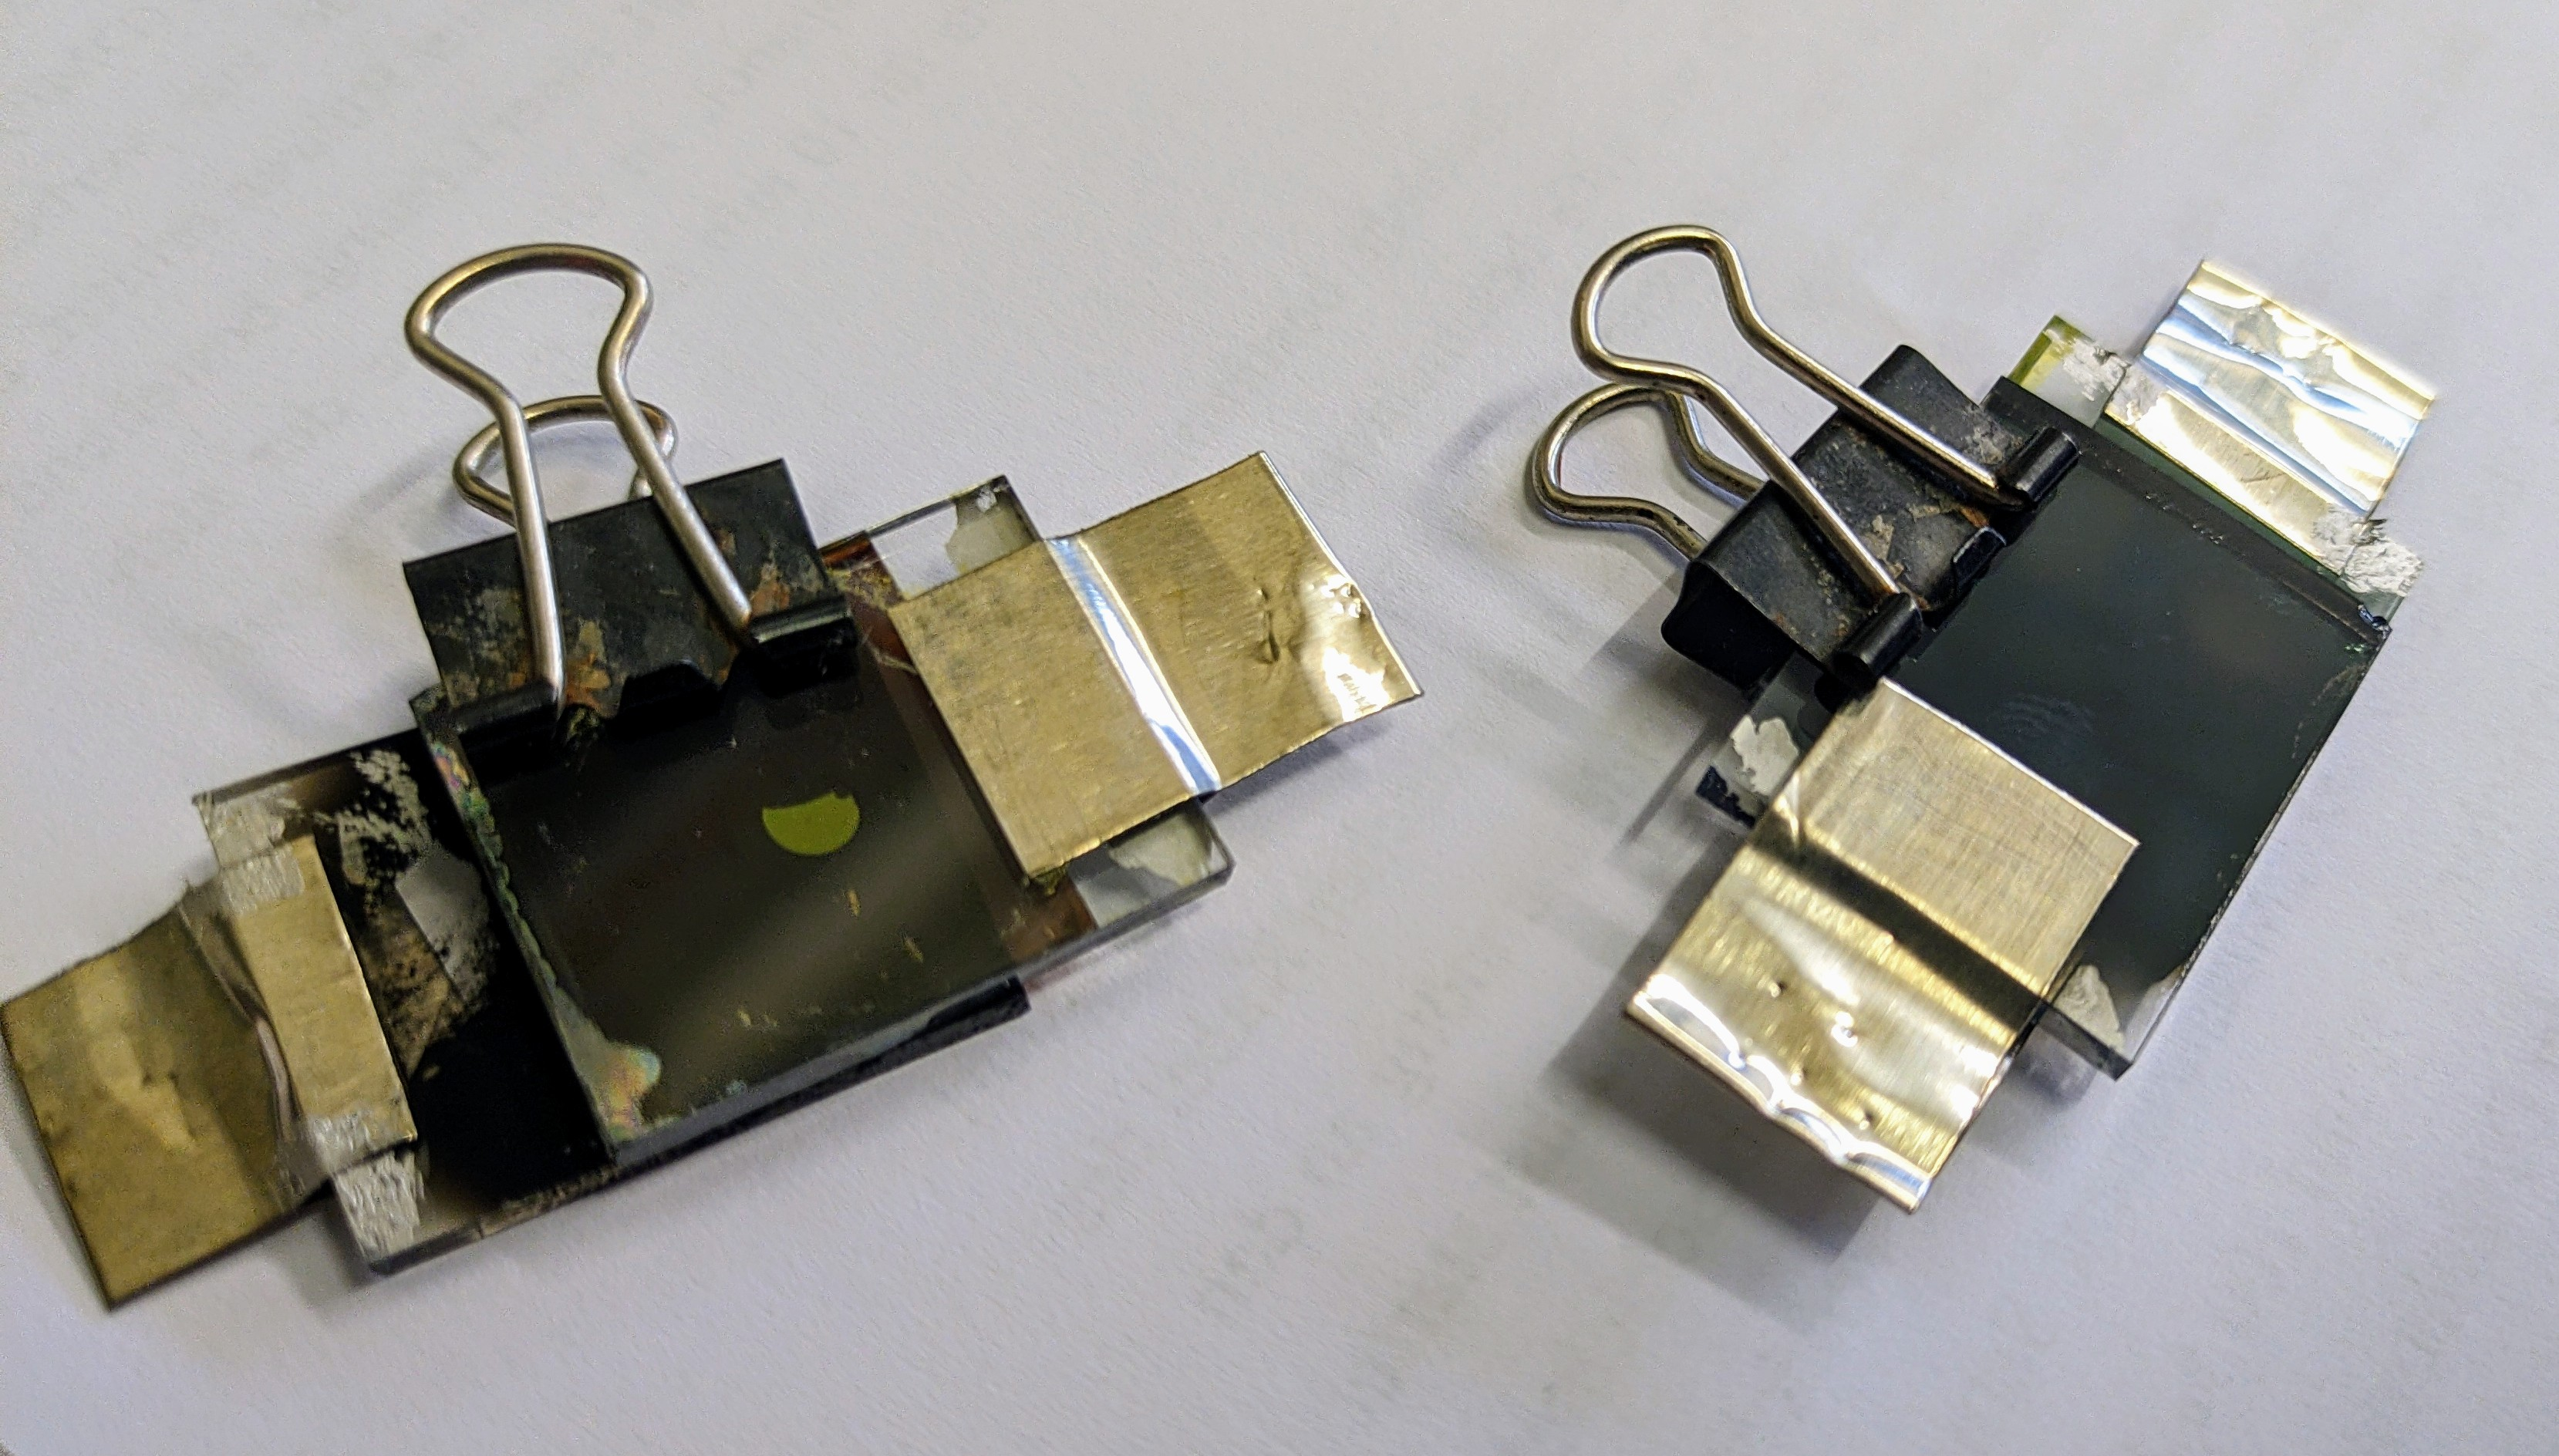
\includegraphics[width=0.8\textwidth]{Bilder/gebauteZelllen.jpg}
			\caption{zusammengebaute Perowskitsolarzellen}
			\label{img:gebauteZellen}
		\end{figure}
	\paragraph{Herstellen der Rückelektrode und Zusammenbau der Solarzelle}	
		Die Rückelektrode wird durch Halten der leitfähigen Seite des FTO-Substrats über eine Flamme rußbeschichtet. Rückelektrode und Probe werden mit Kupferklebeband und Leitsilber kontaktiert. Eine Maske wird auf die Rückseite der Perowskitschicht geklebt, um die belichtete Fläche zu definieren. Die Rückelektrode wird so befestigt, dass kein Kurzschluss entsteht.
		
	\paragraph{Messung von Photoströmen und -spannungen}	
		Zur Messung von Photoströmen und -spannungen wird die Solarzelle mit einer Lichtintensität von \qty{100}{\milli\watt\per\centi\metre\squared} belichtet. Anode und Kathode werden mit Heftklammern  wie in Abbildung \ref*{img:gebauteZellen} zu sehen elektrisch kontaktiert. Die j-V-Kennlinien werden im Dunkeln und unter Belichtung bei verschiedenen Lichtintensitäten gemessen.

		

\chapter{Auswertung}
	\begin{figure}[ht]
		\centering
		\begin{subfigure}[b]{0.45\textwidth}
			\centering
			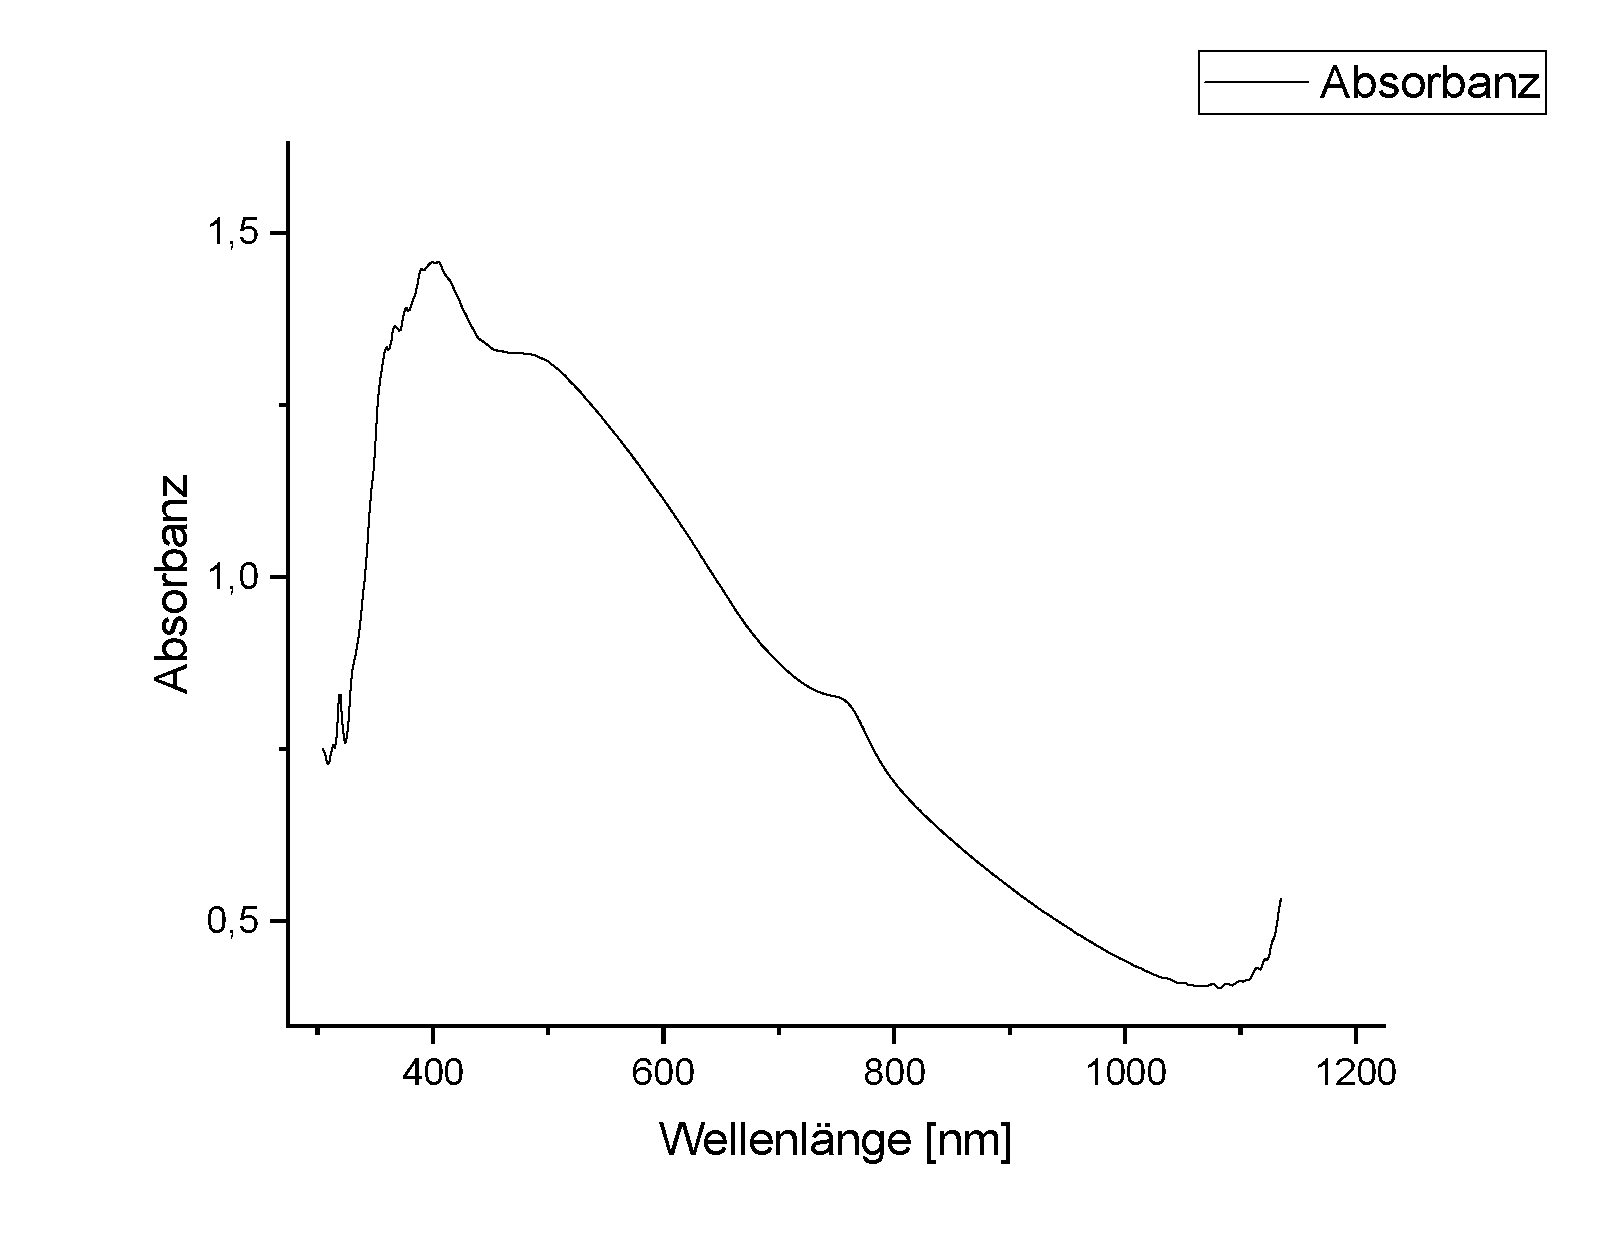
\includegraphics[width=\textwidth]{bilder/AbsP1.pdf}
			\caption{Absorptionsspektrum der ersten Solarzelle}
			\label{fig:AbsP1}
		\end{subfigure}
		\hfill
		\begin{subfigure}[b]{0.45\textwidth}
			\centering
			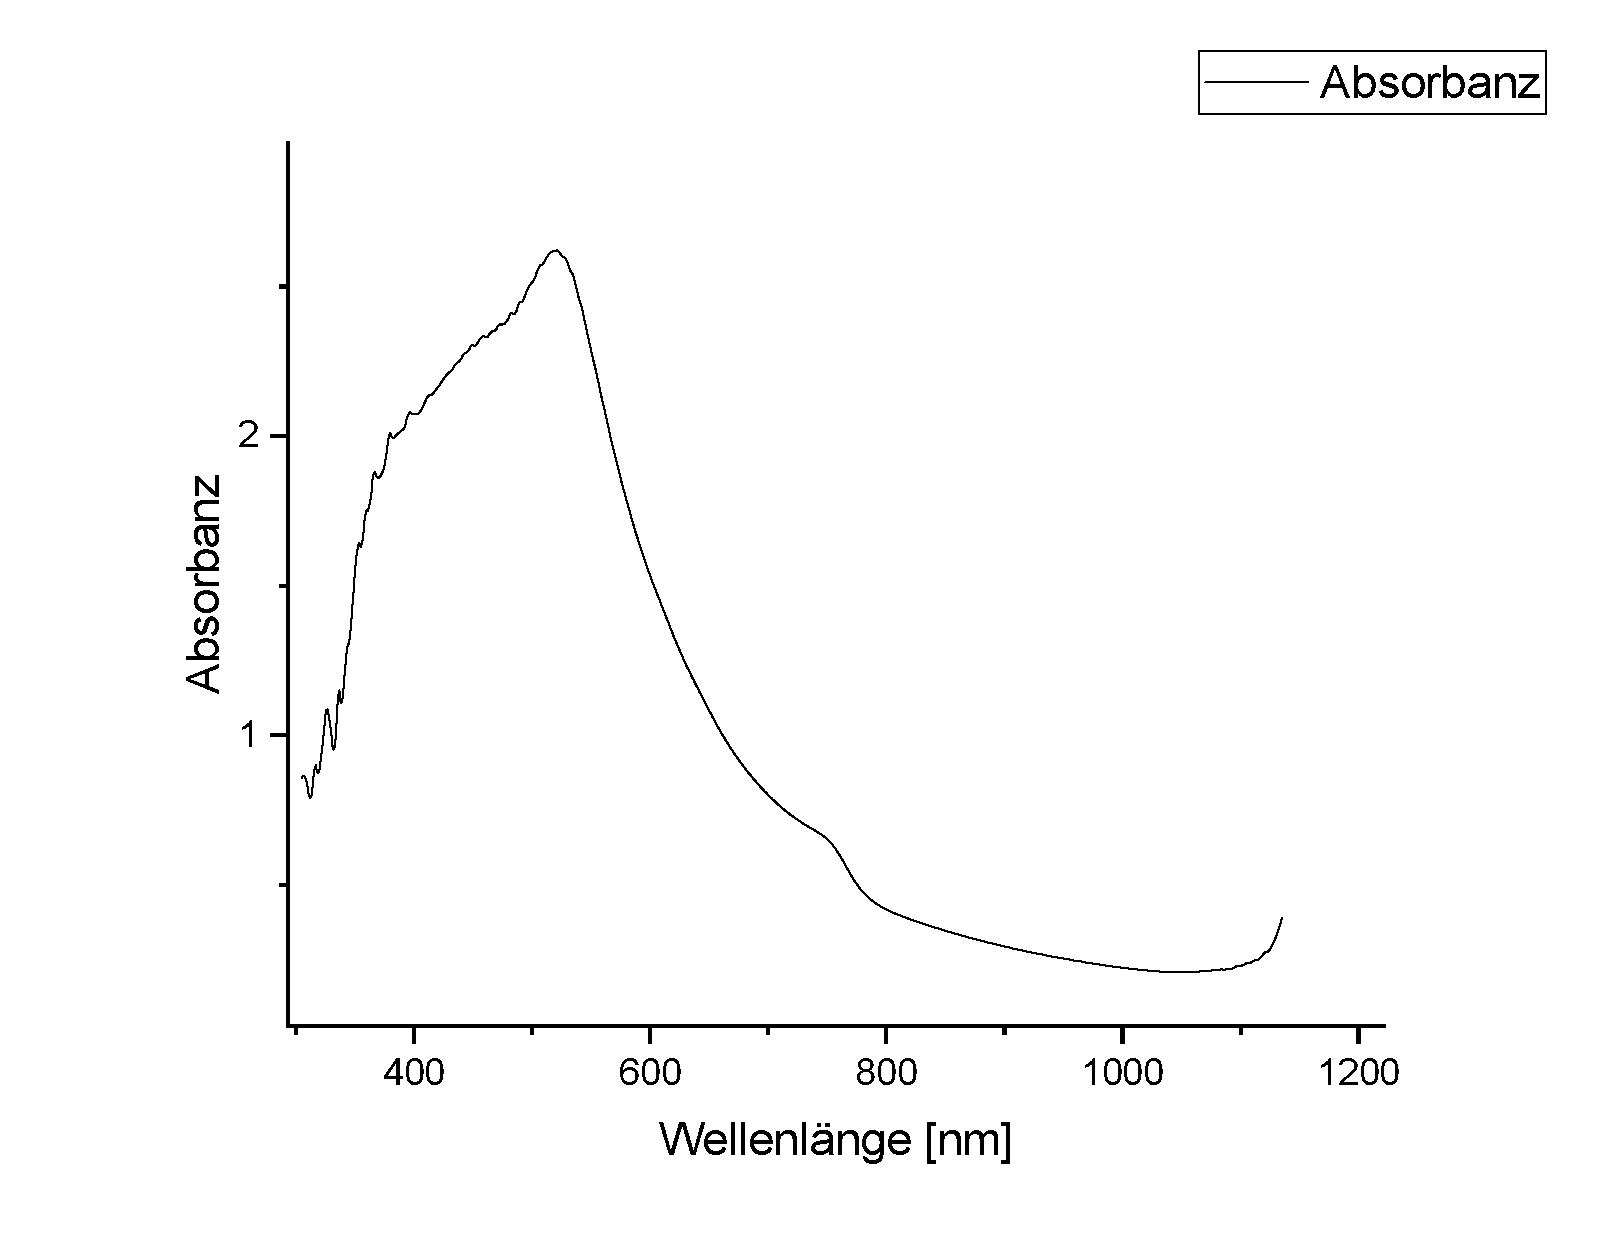
\includegraphics[width=\textwidth]{bilder/AbsP2.pdf}
			\caption{Absorptionsspektrum der zweiten Solarzelle}
			\label{fig:AbsP2}
		\end{subfigure}
		\caption{Absorptionsspektren der beiden Solarzellen}
		\label{fig:AbsP1P2Combined}
	\end{figure}

	\section{Absorptionsspektren}
		Die Absorptionsspektren der beiden Solarzellen sind in Abbildung \ref{fig:AbsP1P2Combined} dargestellt. Die Absorption beginnt bei einer Wellenlänge von etwa \SI{300}{\nano\meter} und steigt bis zu einer Wellenlänge von \SI{400}{\nano\meter} (Solarzelle 1) bzw. \SI{500}{\nano\meter} an. Die Absorptionsspektren zeigen, dass die Perowskitschicht in beiden Solarzellen Licht im sichtbaren Bereich absorbiert. Die Absorption ist bei der zweiten Solarzelle stärker als bei der ersten, was auf eine höhere Absorptionsfähigkeit der Perowskitschicht hinweist. Dies ist ein wichtiger Faktor für die Effizienz der Solarzelle, da eine höhere Absorption mehr Photonen einfängt und somit mehr Elektronen erzeugt.
		Gegen Ende des sichtbaren Bereichs nimmt die Absorption ab, was darauf hindeutet, dass die Perowskitschicht nicht das gesamte Licht absorbiert. Dies könnte auf eine geringere Dicke der Schicht oder eine geringere Absorptionseffizienz zurückzuführen sein.
		Ab \SI{750}{\nano\meter} ist das Absorptionsminimum der Zellen erreicht. Über dieser Energie liefert die Lichtquelle nicht mehr genügend Intensität, um eine aussagekräftige Absorption zu messen, darum steigt die Kurve wieder an. Dies ist jedoch ein Messfehler und keine tatsächliche Absorption.		

	\section{Tauc-Plot}
	\begin{figure}[ht]
		\centering
		\begin{subfigure}[b]{0.45\textwidth}
			\centering
			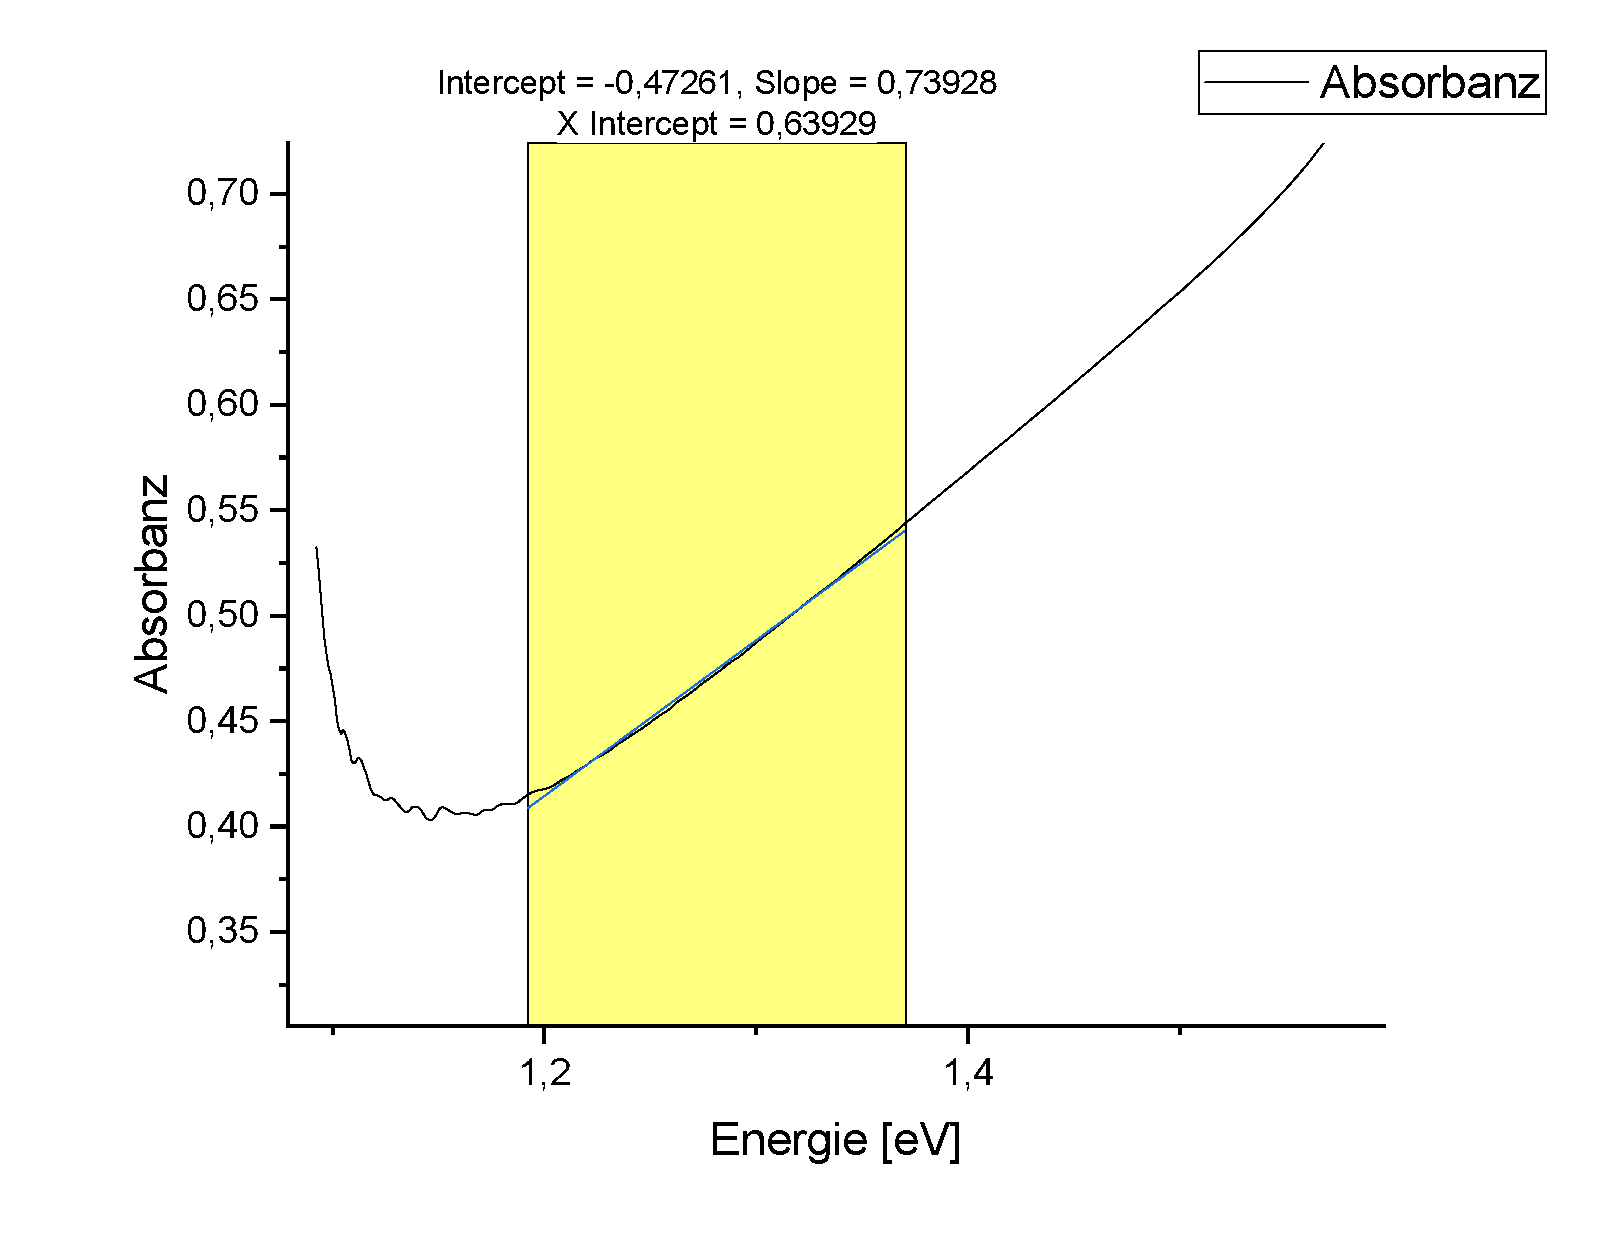
\includegraphics[width=\textwidth]{bilder/TaucP1.pdf}
			\caption{Tauc-Plot der ersten Solarzelle}
			\label{fig:TaucP1}
		\end{subfigure}
		\hfill
		\begin{subfigure}[b]{0.45\textwidth}
			\centering
			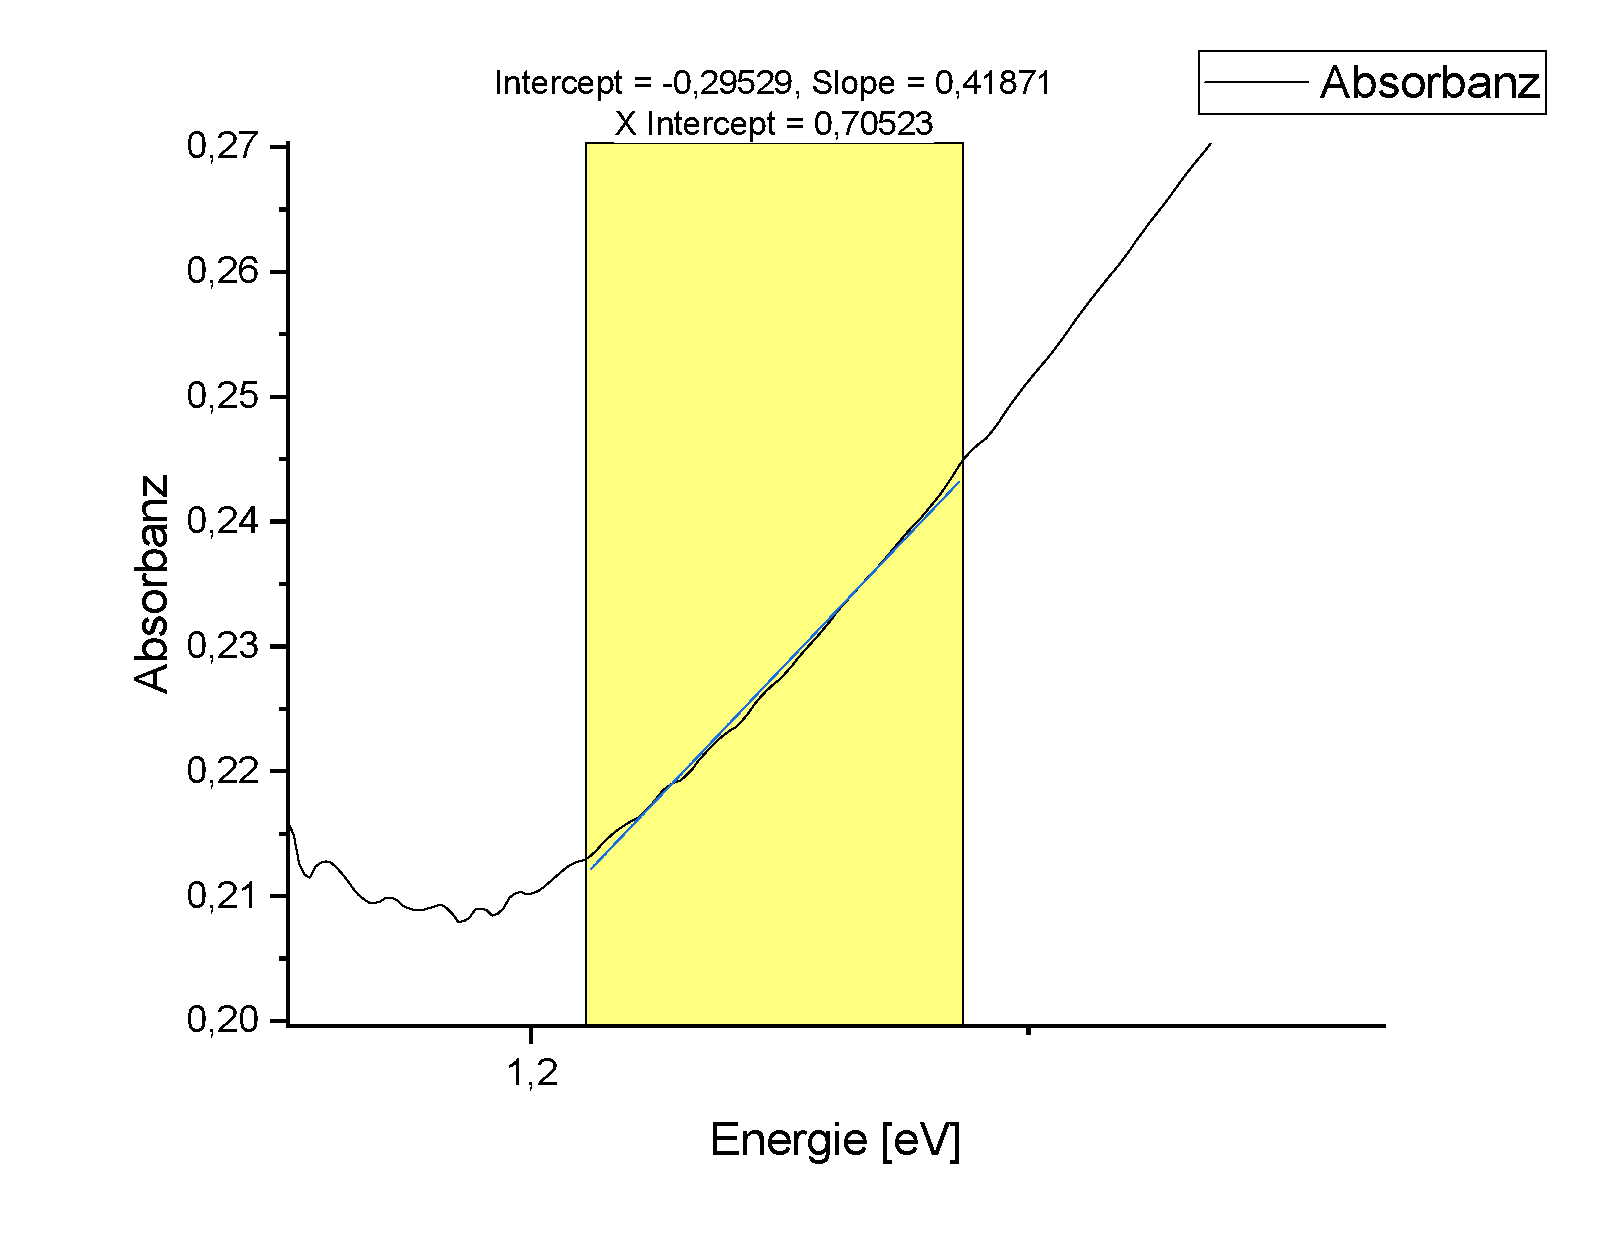
\includegraphics[width=\textwidth]{bilder/TaucP2.pdf}
			\caption{Tauc-Plot der zweiten Solarzelle}
			\label{fig:TaucP2}
		\end{subfigure}
		\caption[Tauc-Plots]{Energie-Absorptionsspektren der beiden Solarzellen mit Tauc-Plot}
		\label{fig:AbsP1P2Combined}
	\end{figure}
		Der Tauc-Plot ist eine Methode, um die Bandlücke eines Halbleiters zu bestimmen. Dazu wird die Absorption gegen die Energie aufgetragen und die Steigung der Geraden im Bereich der Absorptionskante bestimmt. Die Bandlücke entspricht der Energie, bei der die Absorption einen Wert von 0 erreicht. In den Tauc-Plots der Solarzellen sind die Absorptionskanten bei etwa \SI{0,64}{\eV} (Solarzelle 1) und \SI{0,71}{\eV} (Solarzelle 2) zu erkennen. Dies entspricht der Bandlücke des verwendeten Perowskits \ce{CH3NH3PbI3}, die bei \SI{1.55}{\eV} liegt. Die Ergebnisse zeigen, dass die Perowskitschicht in beiden Solarzellen eine direkte Bandlücke aufweist, was für die Effizienz der Solarzelle von entscheidender Bedeutung ist. Jedoch ist die Bandlücke beider Solarzellen viel geringer als die von idealem Perowskit mit circa \SI{1.5}{\eV}. Dies könnte auf eine unvollständige Kristallisation der Perowskitschicht oder eine ungleichmäßige Schichtdicke zurückzuführen sein. Eine geringere Bandlücke führt zu einer geringeren Spannung und damit zu einer geringeren Leistung der Solarzelle. Daher ist es wichtig, die Bandlücke der Perowskitschicht genau zu kontrollieren, um eine hohe Effizienz zu gewährleisten. Die im folgenden Kapitel \ref{ch:Kennlinien} aufgenommenen Kenngrößen der Solarzellen werden die hier zu erwartende geringe Effizienz der Zellen bestätigen.

\section{Charakteristika der Solarzelle}
Beim aufnehmen der Kennlinien hat die hergestellte Solarzelle 1, nur extrem kleine Ströme bei Beleuchtung gezeigt. Die Kennlinien konnten nur in einem minimalen Spannungsbereich aufgenommen werden. Da Solarzelle 2 ein besseres Verhalten gezeigt hat, werden ihre Messdaten im folgenden ausgewertet. Das war in der Auswertung der Tauc-Plots auch zu erwarten, denn die zweite Solarzelle hat eine etwas größere Bandlücke als die erste. \\
\subsection{Kennlinien}\label{ch:Kennlinien}
\begin{figure}
	\centering
	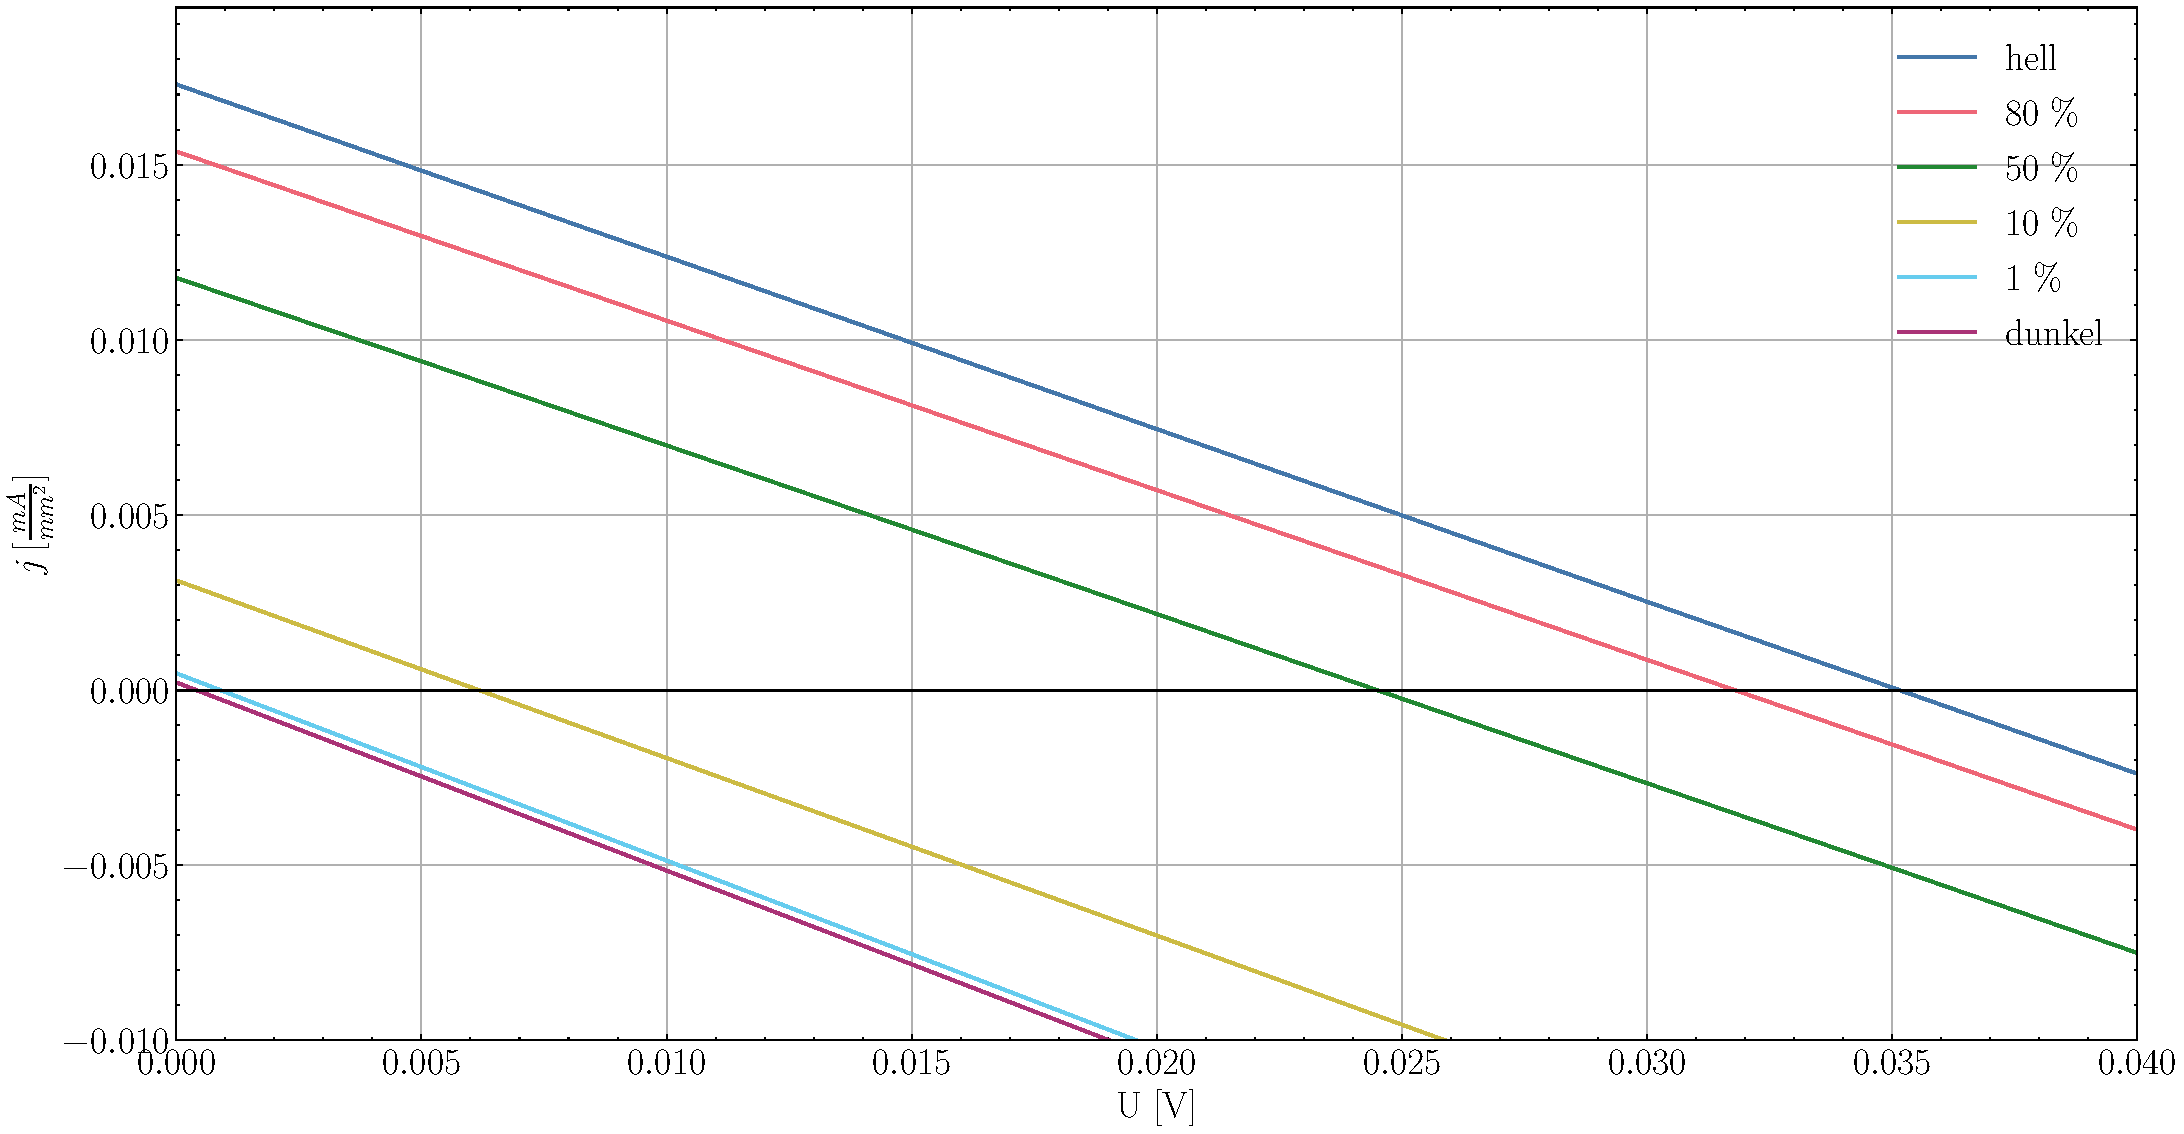
\includegraphics[width=\textwidth]{Bilder/Kennlinien.pdf}
	\caption[Stromdichte-Spannungskennlinien]{Stromdichte-Spannungskennlinien, Dunkel- und Hellkennlinie, zudem Kennlinien bei unterschiedlichen Belichtungsintensitäten}
	\label{img:Kennlinien}
\end{figure}
In Abbildung \ref{img:Kennlinien} sind die Stromdichte-Spannungskennlinien für alle gemessenen Lichtintensitäten aufgetragen. Die y-Achse wird in eine Stromdichte umgerechnet, dies geschieht mit der bekannten beleuchteten Fläche $A$. Diese ist kreisrund und hat einen Durchmesser von \SI{7}{\milli \meter}. Insgesamt sehen alle Linien sehr ohmisch aus, in Abbildung \ref{img:KennlinienLOG} ist zu erkennen, das die Solarzelle dennoch minimal ein Diodenverhalten ausweist. Denn bei logarithmischer y-Achse ist die typische Form, wie sie im Theoriekapitel \ref{ch:Kenngrößen} beschrieben wurde, erkennbar.\\
Ab einer Beleuchtungstärke von 10 \% und mehr, liegt ein Teil der Graphen im positiven Bereich der y-Achse, demzufolge wird tatsächlich Leistung erzeugt, die Solarzelle funktioniert also prinzipiell.\\
Durch lineare Interpolation werden die Kurschlussstromdichten und Leerlaufspannungen bestimmt, Stromdichten werden über die Fläche wieder in Ströme umgerechnet. Die Ergebnisse daraus sind in Tabelle \ref{table:KurzschlussLeerlauf} aufgetragen. 
\begin{table}[h!]
	\centering
	\begin{tabular}{c c c c}
		\toprule[1.5pt]
		Beleuchtung & $V_{OC}$ [\si{\milli \volt}] & $j_{SC}$ [\si{\milli \ampere \per \milli \meter \squared}] & $I_{SC}$ [\si{\milli \ampere}] \\
		\midrule
		hell        & 35.15  &  0.01729  & 1.353      \\
		80 \%       & 31.79  &  0.01537  & 1.223            \\
		50 \%       & 24.45  &  0.01176  & 0.943            \\
		10 \%       & 6.17   &  0.00313  & 0.237          \\
		1  \%       & 0.89   &  0.00048  & 0.034          \\
		dunkel      & 0.40   &  0.00022  & 0.016          \\
		\bottomrule[1.5pt]
	\end{tabular}
	\caption{Kurschlussstromdichten und Leerlaufspannungen}\label{table:KurzschlussLeerlauf}
\end{table}
\begin{figure} 
	\centering
	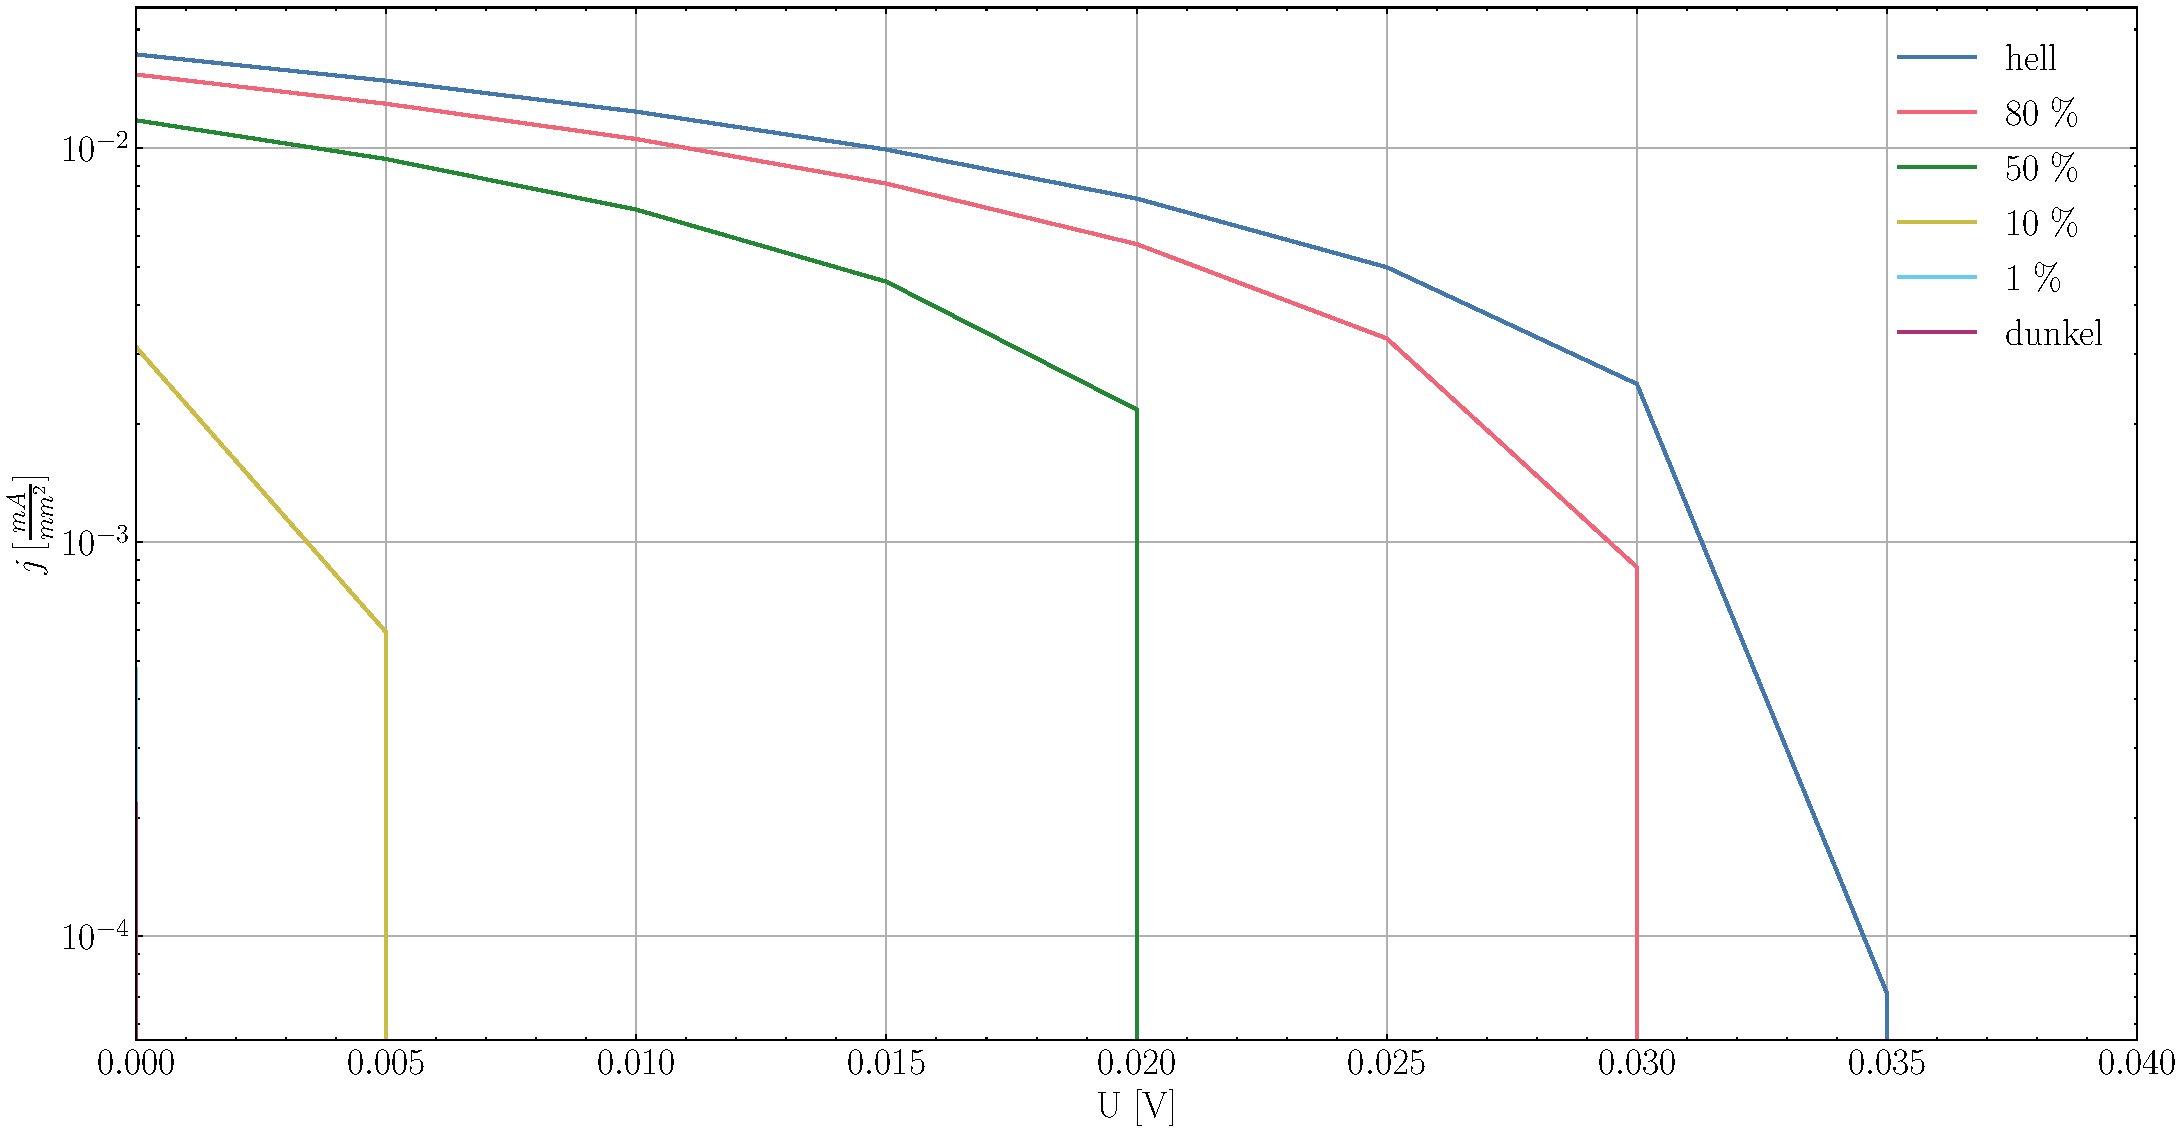
\includegraphics[width=\textwidth]{Bilder/KennlinienLOG.pdf}
	\caption{Logarithmische Stromdichte-Spannungskennlinien}
	\label{img:KennlinienLOG}
\end{figure}
\chapter{Fazit}
	\fehlt

\listoffigures%\addcontentsline{toc}{chapter}{\listfigurename}
	
\begin{thebibliography}{111}%\addcontentsline{toc}{chapter}{Literaturverzeichnis}
	\bibitem{Anleitung}
	Anleitung zum Fortgeschrittenen"~Praktikum.\\ \glqq Versuch:\.Organisch"~anorganisch hybride Perowskitsolarzellen\grqq.\\ Justus-Liebig-Universität Gießen. Sommersemester 2024.
	
	\bibitem{Boix}
	Boix, P. P., Nonomura, K., Mathews, N., \& Mhaisalkar, S. G. (2014). Current progress and future perspectives for organic/inorganic perovskite solar cells. Materials Today, 17(1), 16–23. doi:10.1016/j.mattod.2013.12.002.

	\bibitem{Grätzel}
	Grätzel, M. (2014). The light and shade of perovskite solar cells. Nature Materials, 13(9), 838– 842. doi:10.1038/nmat4065.
	\bibitem{Kojima}
	Kojima A et al. (2009). Organometal Halide Perovskites as Visible-Light Sensitizers for Photovoltaic Cells.
	Journal of the American Chemical Society. DOI: 10.1021/ja809598r.
	
	\bibitem{Sharma}
	Sharma R et al. (2022): Stability and efficiency issues, solutions and advancements in perovskite solar cells: A review. Solar Energy. DOI: 10.1016/j.solener.2022.08.001.

	\bibitem{NREL}
	National Renewable Energy Laboratory (NREL). Best Research-Cell Efficiencies.

	\bibitem{Green}
	Green MA et al. (2019). Solar cell efficiency tables (version 55). Progress in Photovoltaics: Research and Applications. DOI: 10.1002/pip.3171.

	\bibitem{Holzhey}
	Holzhey P et al. (2023): Toward commercialization with lightweight, flexible perovskite solar cells for residential photovoltaics. Joule. DOI: 10.1016/j.joule.2022.12.012.

	\bibitem{Perovskite}
	Perovskite-Info. The Perovskite Handbook. URL: \url{https://www.perovskite-info.com/}.
	
	\end{thebibliography}


% \chapter*{Anhang}\label{ch:Anhang}\addcontentsline{toc}{chapter}{Anhang}
% \FloatBarrier
% 	\begin{figure}[ht]
% 	\centering
% %	\includegraphics[width=\textwidth]{data/Testat.pdf}		
% 	\caption[Testat]{Das Testat des Versuchs}
% 	\label{fig:Testat}
% \end{figure}

\end{document}
